
\chapter{Localization\label{ch:localization}}

\section{Problem Description}
	For a robot to perform precise maneuvers, it must first have an understanding of its position and orientation, or pose. This is the problem of localization. By using a variety of sensor measurements, the localization algorithm must produce a single estimate of the quadcopter's pose for use in the controller.

\section{Considerations of the AR.Drone}

	As this project uses the AR.Drone 2.0, the localization algorithm is built around the capabilities and limitations of this hardware. Considering the low load-capacity of the AR.Drone and the fact that this project aims to use off-the-shelf hardware, the localization algorithm may only use the sensors included in the AR.Drone.

	Therefore, the localization must produce an estimate by using some combination of the forward camera, downward camera, accelerometer, gyroscope, magnetometer, ultrasound altimeter, and pressure altimeter. 

\section{Localization Methods}

	Localization for mobile robots fall into three main categories: Kalman, Grid-Based, and Monte Carlo.

	%ASK: How do Kalman filters work?
	\subsection{Extended Kalman Filter}
	The extended Kalman Filter (EKF) is used extensively in mobile robot localization. The EKF is a nonlinear version of the Discrete Kalman Filter first introduced by Rudolf Emil Kalman in 1960~\cite{Kalman}. The EKF linearizes about the current mean and covariance in  method similar to a Taylor series. The EKF contains two stages, a prediction step and a correction step. In the prediction step, the new state and error covariance are projected. Then, in the correction step, the estimate and error covariance are updated in response to sensor measurements~\cite{Welch}. However, Kalman filters have the disadvantage of only being able to approximate normal distributions.

	%I need a better reason why I am not using Kalman filter
	\subsection{Grid-Based Markov Localization}
	Grid-based localization uses a ``fine grained'' grid approximation of the belief space, that is the space that covers all of the potential position and orientations of the robot~\cite{Fox}. For each time step, the probability of a robot being in any one of the grid cells is calculated, first by using odometry and then by exteroceptive sensors such as range finders. While relatively straightforward to implement, this process has many drawbacks. First of all, picking the size of the grid cells can be difficult. If the cells are too large, then the estimate will not be precise. However, if the cells are too small, the algorithm will be slow and very memory-intensive. Additionally, grid-based localization performs poorly in higher-dimensional spaces, as the number of cells grows exponentially with the number of dimensions.

	\subsection{Particle Filter}
	A particle filter is a type of Monte Carlo simulation with sequential importance sampling~\cite{Alkhatib}. Essentially, a particle filter keeps track of a large number of particles, which represent possible pose estimation. The particle filter typically moves these particles using proprioceptive sensor measurements convolved with Gaussian noise~\cite{Fox}. Then, the particles are weighted with respect to exteroceptive sensor measurements. These particles are then randomly resampled based on these weight values, producing a corrected distribution of particles.

	There are many advantages to using a particle filter. Due to the way the process creates an approximation by a set of weighted samples without any explicit assumptions of the approximation's form, it can be used in applications where the assumption of Gaussian noise doesn't necessarily apply~\cite{Alkhatib}.

\section{Particle Filter with Augmented Reality Tags}

	\begin{algorithm}
		\centering
		\caption{Particle Filter with Augmented Reality Tag Correction} 
		\begin{algorithmic}[1]
			\ForAll {$t$}
				\If{\textit{buffer\_full()}}
					\State{\textit{predict}$(\Delta t, v_x, v_y, altd, \theta)$}
				\EndIf
				\If{$recieved\_tag()$}
					\State {\textit{correct}$(\textbf{P})$} \Comment{Transformation matrix from camera to marker}
				\EndIf
				\State {$\textbf{x}_{est} \gets $\textit{get\_estimate()}}
			\EndFor
		\end{algorithmic}
	\end{algorithm}

	%Provide a brief background on the origination of the particle filter, uses, advantages, etc.
	The particle filter has been chosen for this project due to its flexibility, ease of implementation, and performance. In typical implementations of particle filters for mobile robots, the prediction step uses proprioceptive sensors, such as accelerometers, gyroscopes, and rotary encoders. Then, this estimate is typically corrected by using exteroceptive sensors, such as infrared, laser, or ultrasound.

	However, due to the lack of horizontal range sensing, this particle filter uses a different division between the prediction and correction steps. The prediction step uses the stock configuration of sensors in the AR.Drone, specifically the fused velocity, gyroscope, and ultrasound altimeter measurements. Then, the correction step uses an estimated global position determined by augmented reality tags to resample the particles.


	\subsection{Buffering Navdata}

		The localization module receives navdata at 50Hz. Depending on the number of particles and computational resources available to the localization algorithm, this can be a higher rate than the particle filter can run the propagation step. Reducing the rate at which propagation is run allows the particle filter to use more particles, providing better coverage of the pose estimate space and increasing the likelihood of convergence.

		Additionally, while a more rapidly updated pose estimate would be preferable, the accuracy of the measurement is not such that it is especially useful to update at a rate of 50Hz. For example, the maximum velocity that the quadcopter should ever achieve in this system is around 500mm/s. In .02 seconds, the quadcopter will have only moved 10mm, or 1cm. Considering that the desired accuracy of the localization is on the order of tens of centimeters, updating the estimated pose at a reduced rate is acceptable.

		As the navdata is recieved, the navdata measurements, such as velocity and yaw, are added to a buffer of size $n$. Every $n$ measurements, the propagate step is called with the simple moving average of the previous $n$ values and the sum of the $\Delta T$ values since the last call to propagate. This results in a propagate rate of $50/n$Hz.

		Although the buffer size is currently a hard-coded value, this could be dynamically changed based on the amount of delay between receiving navdata measurements and processing them in the propagate step. This would result in the highest propagate rate possible given a fixed number of particles. On the other hand, the buffer size could remain fixed with the particle filter adjusting the total number of particles, allowing for the best possible coverage at a guaranteed update rate.

	\subsection{Initialization}

		The particle filter is initialized by creating a set of $N$ particles. Each of these particles represents a potential pose in the configuration space. In particular, each particle at a given time step $t$ is of the form:

		\[\textbf{x}_t = \begin{bmatrix} 
			  x_t\\
			  y_t\\
			  z_t\\
			  \theta_t\\
			\end{bmatrix}	
		\]

		Where $x_t, y_t, z_t$ are the position, in mm, and $\theta_t$ is the heading, in degrees, of the particle in the global coordinate space. As the low level stabilization and control of the quadcopter is handled by the on-board processor, it is not necessary to include roll and pitch in the pose estimate of the quadcopter as these are not needed for the high level control. The entire set of particles of size $N$ at time step $t$ can be described as:

		\[
		\textbf{X}_t = [\textbf{x}_t[0], \textbf{x}_t[1],...,\textbf{x}_t[N]]^T
		\]

		Additionally, for each time step, there is a set of associated weights

		\[
		\textbf{W}_t = [w_t[0], w_t[1],...,w_t[N]]^T
		\]

		Normalized, such that

		\[
		\sum_{i=0}^N w_t[i] = 1
		\]


		\subsubsection{Coordinate Frame Conventions}

			\begin{figure}
			\centering
				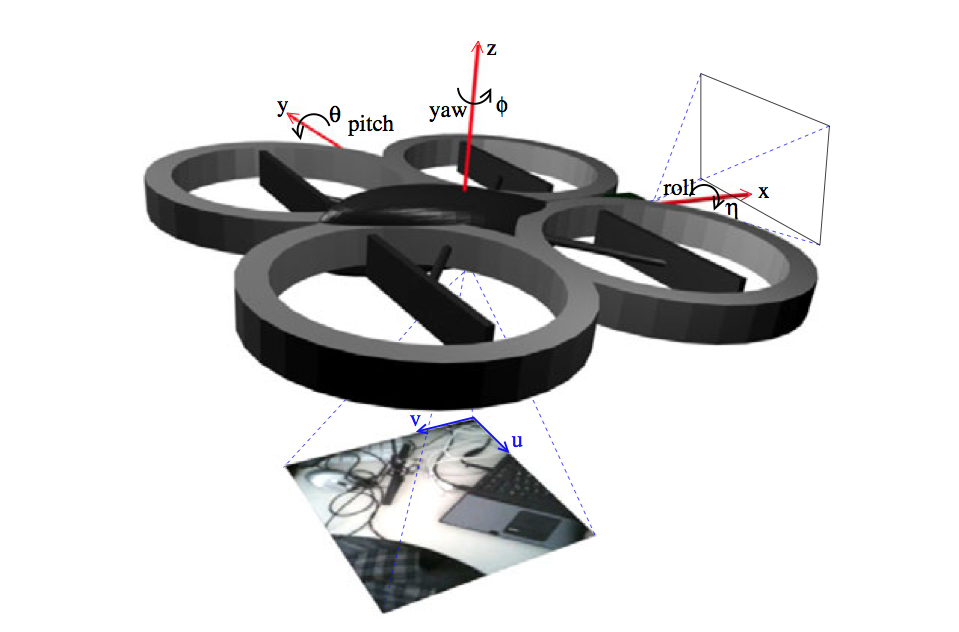
\includegraphics[width=300px]{../images/coordinates.png}
				\caption{AR.Drone Coordinate System~\cite{ARDroneEducation}.}\label{fig:coords}
			\end{figure}

			The coordinate frame follows the standard set by the ardrone\_autonomy package. As shown in Figure~\ref{fig:coords}, the coordinate frame is right-handed, with positive $x$ as forward, positive $y$ as left, and positive $z$ as up. In terms of rotation, a counter clockwise rotation about an axis is positive. Heading ranges from -180 degrees to 180 degrees, with 0 centered along the $x$-axis. When the particle filter is initialized, the global coordinate frame is set equal to the first instance of the local coordinate frame.


	\subsection{Prediction Step}

		\begin{algorithm}
			\centering
			\caption{Prediction Step} 
			\begin{algorithmic}[1]
				\Function{Predict}{$\Delta t, v_x, v_y, \theta, z_{\textit{ultra}}$}
					\State {$\Delta\theta \gets \theta -  \theta_{t-1}$}
					\For {$i=0 \to N$}
						\State {$\Delta\theta_{\textit{noise}} \gets \textit{randn}(\Delta\theta, \sigma_{\theta})$} 
						% \Comment{$randn(\mu, \sigma)$ returns a normally-distributed random value}
						\State {$\theta_{t}[i] \gets  \theta_{t-1}[i] + \Delta\theta_{\textit{noisy}}$} \label{predict:line:theta}
						\State {$(v_{\textit{x,global}} , v_{\textit{y,global}}) \gets \textit{transform}(v_x, v_y, \theta_{t}[i])$} \label{predict:line:transform}
						\State {$v_{\textit{x,global,noisy}} \gets \textit{randn}(v_{\textit{x,global}}, \sigma_{v})$}
						\State {$v_{\textit{y,global,noisy}} \gets \textit{randn}(v_{y,global}, \sigma_{v})$}
						\State {$x_{t}[i] \gets \Delta t*v_{\textit{x, global, noise}} + x_{t-1}[i]$} \label{predict:line:position}
						\State {$y_{t}[i] \gets \Delta t*v_{\textit{y, global, noise}} + y_{t-1}[i]$}
						\State {$z_{t}[i] \gets \textit{randn}(z_{\textit{ultra}}, \sigma_{ultra})$}
					\EndFor
				\EndFunction
			\end{algorithmic}
		\end{algorithm}

		The first component of a particle filter is the prediction step. In this step, the position of every particle is updated by using the sensor measurements contained in the navdata messages. Specifically, the prediction step uses the elapsed time, $\Delta t$, fused velocity measurements, $v_x$ and $v_y$, yaw reading, $\theta$, and ultrasound altimeter value, $z_{ultra}$.

		The prediction step then subtracts the value of $\theta_{t-1}$, the value of theta from the previous estimate, from $\theta$ to produce $\Delta\theta$. Then, for every particle $i$, a new pose $\textbf{x}_t[i]$ is generated using the previous pose, $\textbf{x}_{t-1}[i]$ and the values $\Delta t, v_x, v_y, \Delta\theta,$ and $z_{ultra}$.

		\subsubsection{Adding Noise to Sensor Measurements}
			In order to update the pose estimation for a given particle, noise is first added to the sensor measurements in order to model the sensor noise. By adding noise to the particles, the distribution of particles should expand to include all of the possible belief states.

			%INCLUDE A GRAPHIC SHOWING THE SPREADING OUT OF PARTICLES OVER TIME

			For each sensor value, a new ``noisy'' value is generating by a sampling from a Gaussian distribution with a mean of the sensor reading and a standard deviation, $\sigma$, which models in accuracy of the sensor. 
		
		\subsubsection{Converting Local Velocity to Global Velocity}
			In order to update the pose of each particle in the global frame, the values $v_{\textit{x,noisy}}$ and $v_{\textit{y,noisy}}$, must be transformed from the local coordinate frame of the quadcopter to the global coordinate frame. First, on Line~\ref{predict:line:theta}, the new heading of the particle is determined by adding the value $\Delta\theta_{\textit{noisy}}$ to the estimated heading of the last time step, $\theta_{t-1}[i]$.

			Then, on Line~\ref{predict:line:transform}, the global velocity is found by
			\[
			\begin{bmatrix} 
			  v_{\textit{x,global,noisy}}\\
			  v_{\textit{y,global,noisy}}\\
			\end{bmatrix}
			=
			\begin{bmatrix} 
			  cos(\theta_t[i]) & -sin(\theta_t[i])\\
			  sin(\theta_t[i]) & cos(\theta_t[i])\\
			\end{bmatrix}
			\begin{bmatrix} 
			  v_{\textit{x,noisy}}\\
			  v_{\textit{y,noisy}}\\
			\end{bmatrix}
			\]

		\subsubsection{Position Update}
			Once the velocity is in the global coordinate frame, Euler integration is used on Line~\ref{predict:line:position} to determine the new position of the particle.

	\subsection{Correction Step}
		
		\begin{spacing}{2.0}
		\begin{algorithm}
			\centering
			\caption{Correction Step} 
			\begin{algorithmic}[1]
				\Function{Correct}{$\textit{marker\_id}, \textbf{P}$} \Comment{$\textbf{P}$ is transformation from camera to marker}
				\\
				\State{$\textbf{M} \gets \textit{lookupTransform(world, marker\_id)}$} 
				% \Comment{Transformation between world and tag}
				\State{$\textbf{B} \gets \textit{lookupTransform(base, camera)}$} 
				% \Comment{Transformation between quadcopter base an camera}
				\State{$\textbf{T} \gets \textbf{M}\textbf{P}^T\textbf{B}^T $}\label{correct:line:transformation}
				\State{$(x_{\textit{correct}}, y_{\textit{correct}}, z_{\textit{correct}}) \gets \textit{getTranslation}(\textbf{T})$}\label{correct:line:gettranslation}
				\State{$\theta_{\textit{correct}} \gets \textit{getHeading}(\textbf{T})$}\label{correct:line:getrotation}

				\\
				\\
				\State{$w_{sum} \gets 0$}
				\For{$i=0 \to N$} \Comment{Weighting Particles}
					\State{$\textit{dist} \gets \sqrt{(x_{t}[i]-x_{\textit{correct}})^2 + (y_{t}[i]-y_{\textit{correct}})^2 + (z_{t}[i]-z_{\textit{correct}})^2} $}\label{correct:line:euclid}
					\State{$\theta_{\textit{diff}} \gets |\theta_{t}[i] - \theta_{\textit{correct}}| $}\label{correct:line:theta}
					\State{$w_{\textit{dist}} \gets \textit{pdf}(\textit{dist}, 0, \sigma_{x, \textit{artag}})$}\label{correct:line:pdf}
					\State{$w_{\theta} \gets pdf(\theta_{diff}, 0, \sigma_{\theta,\textit{artag}})$}
					\State{$w_t[i] \gets w_{\textit{dist}} + w_{\theta} $}
					\State{$w_{\textit{sum}} \gets w_{\textit{sum}} + w_t[i]$}
				\EndFor

				\\
				\\
				\For{$i=0 \to N$} \Comment{Normalizing Weights}
					\State{$w_t[i] \gets w_t[i]/w_{\textit{sum}}$}
				\EndFor

				\\
				\\
				\State{$\textit{walkerInitialize}(\textbf{X}_t, \textbf{W}_t)$}
				\For{$i=0 \to N$}
					\State{$\textit{randVal} \gets \textit{rand}(0, 1)$}
					\If{$\textit{randVal} < \textit{resampleThreshold}$} \Comment{Random Resampling}
						\State{$x_{\textit{new}} = [x_{\textit{correct}}, y_{\textit{correct}}, z_{\textit{correct}}, \theta_{\textit{correct}}]^T$}
					\Else \Comment{Weighted Sampling of Particles}
						\State{$x_{\textit{new}} = \textit{walkerSelect()}$}
					\EndIf
					\State{$\textbf{X}_{\textit{temp}} \gets \textbf{x}_{\textit{new}}$}
				\EndFor

				\\
				\\
				\State{$\textbf{X}_t \gets \textbf{X}_{temp}$}
				\Comment{Copy new set of particles}
				\\
				\EndFunction
			\end{algorithmic}
		\end{algorithm}
		\end{spacing}

		\subsubsection{Determining Global Position from Augmented Reality Tag}
			The main concept in the correction step is to use a known marker position and a calculated camera-to-marker transformation in order to determine the global position of the quadcopter. Using this calculated global position, the particles, weighted by their similarity the calculated global position, are resampled to correct for the drift accumulated by using local measurements.

			The first step is to determine the pose of the quadcopter in the global coordinate frame using augmented reality tags. These tags, each with unique binary patterns, are placed in known positions and orientations (e.g. axis aligned in the corners of a 5m square). These positions are published as ROS static transforms, allowing them to be retrieved by a \textit{lookupTransform()} command. When a tag is detected by the \texttt{ar\_pose} library, a marker is published containing the id of the tag and the transformation matrix from the camera to the tag, $\textbf{P}$. Then, the transformation matrices from the world frame to the tag,$\textbf{M}$,  and from quadcopter base to camera,$\textbf{B}$, are retrieved using \textit{lookupTransform()}. Through matrix multiplication, the transformation from world to quadcopter, $\textbf{T}$, can be obtained as follows:

			\[\textbf{T} = \textbf{M}\textbf{P}^T\textbf{B}^T \]

			On lines~\ref{correct:line:gettranslation} and~\ref{correct:line:getrotation}, the ROS transformation library is used to derive the estimated position and orientation of the quadcopter, $x_{correct}$, from the transformation matrix $\textbf{T}$.

		\subsubsection{Weighting Particles}
			Each particle is assigned a weight by comparing the particle pose, $x_t[i]$, to the pose estimate generated using the augmented reality tag, $x_{correct}$. First, the Euclidean distance between the two positions and the difference between $\theta$ estimates are calculated on lines \ref{correct:line:euclid} and~\ref{correct:line:theta}.

			Then, on line~\ref{correct:line:pdf}, position and orientation weights are determined by inputing \textit{dist} and \textit{diff} into zero-mean probability density functions with standard deviations derived from testing.

			$pdf(x, \mu, \sigma)$ is defined as:

			\[ \frac{1}{\sigma\sqrt{2\pi}}e^{-\frac{1}{2}(\frac{x-\mu}{\sigma})^2} \]
			
			Where

			\begin{table}[H]
				\centering
			\begin{tabular}{@{}r@{$\quad$\,}l}
				$x$ & Input value\\
				$\mu$ & Mean of normal distribution\\
				$\sigma$ & Standard deviation of normal distribution
			\end{tabular}
			\end{table}

		 
		\subsubsection{Random Resampling}

			Every time the correction step is called, a small percentage of particles are replaced using the pose as estimated by using the augmented reality tags. As the quadcopter will often fly for several meters without picking up a tag, the particles will become very spread out to account for sensor drift. Without replacement, there is a chance that the quadcopter would not be able to recover from a large amount of drift as no particle would be close enough to the actual position to accurately correct. By resampling, the particles will more rapidly cluster when the quadcopter is over a tag. There is a tradeoff of doing this, however. On rare occasions, the \texttt{ar\_pose} library mistake the $marker\_id$ of the tag, resulting in an incorrect transformation. If the resample rate is too high, then a large number of particles will essentially ``teleport'' to the wrong position, resulting in a large jump of estimated pose. If this resample rate is small enough, then it will still accomplish the goal of quickly clustering particles when above tags, but will be robust enough to recover from incorrect tag transformations.


		\subsubsection{Weighted Sampling of Particles}

			The rest of the particles are chosen using a weighted sampling. Essentially, particles that are closest to the position calculated using the augmented reality tags will be chosen with a higher probability, allowing other particles to die out. This is often called ``survial of the fittest'' sampling. The naive method of performing weighted sampling would be to keep an array of cumulative weights. This way, a random number generated between 0 and 1 could be used to search through the array and pick particles with the correct distribution. This would result in a lookup time of $O(\log{N})$ However, using Walker's alias method, a small amount of preprocessing can reduce these lookups to $O(1)$~\cite{Walker}. As there are many particles and the correction step can be called at a very high frequency, it is important to reduce the lookup time as much as possible.

	\subsection{Pose Estimate from Particles}
		At the end of call to the localization algorithm, a new pose estimate is generated using the particle distribution. This is done by taking a linear combination of all of the particles. This method works reasonably well for this application as the particles tend to stay in a single cluster. In applications where multiple belief clusters are likely to exist, such as in a particle filter with an unknown start position, this solution would not be sufficient and a technique such as mean shift clustering should be used. 


